\documentclass[../../main.tex]{subfiles}

\begin{document}

\section{Considerazioni sulla dashboard del DPC}\label{s:considerazioni}
Apriamo questa sezione con uno screenshot della dashboard del DPC effettuato in data 17 febbraio '21.

\begin{figure}[h]
    \centering
    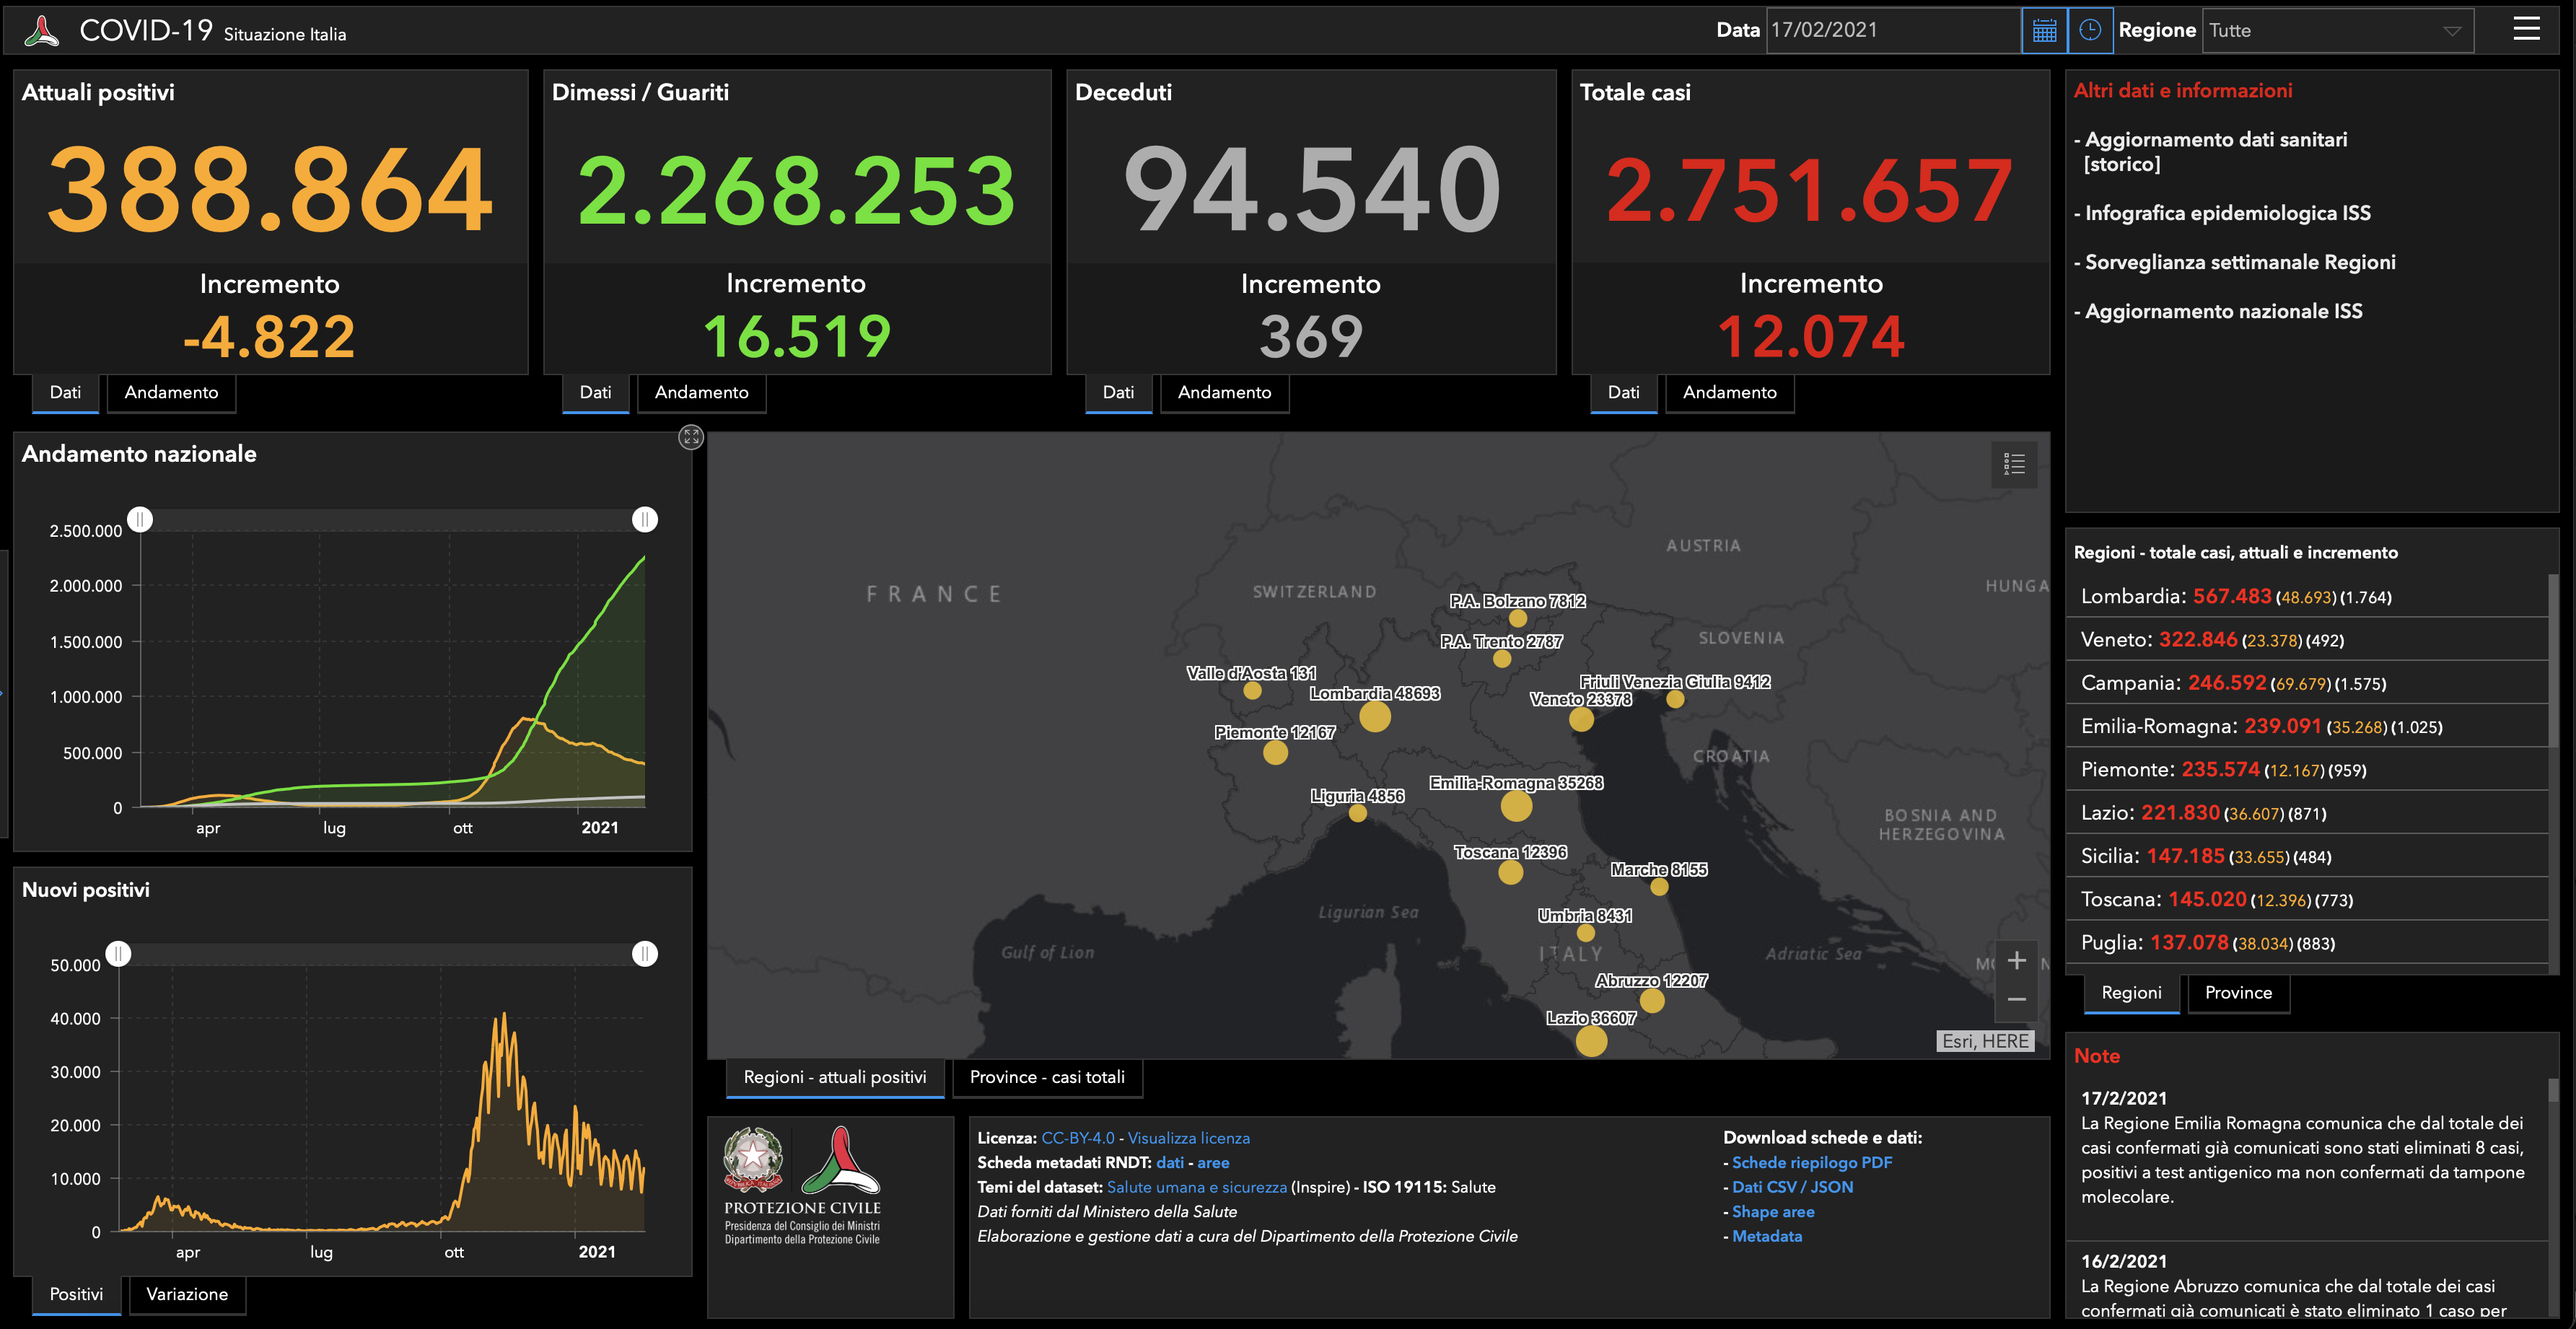
\includegraphics[width = \textwidth]{screenshot-dashboard-DPC}
    \caption{Screenshot della dashboard del Dipartimento della Protezione Civile catturato il 17 febbraio '21.}
    \label{fig:screen-dashboard-DPC}
\end{figure}

Di seguito riportiamo le principali criticità riscontrate, articolandole in due parti: la prima si riferisce agli aspetti estetici e strutturali che minano l'usabilità complessiva e concorrono ad una scadente esperienza utente, mentre la seconda attiene alle carenze nel contenuto informativo e nelle funzionalità che ne riducono il raggio di utilità.

\subsection{Criticità nell'esperienza utente}\label{ss:criticita}
\begin{enumerate}
    \item \textbf{Dimensione eccessivamente piccola di alcune scritte}: il riferimento è ai due box, uno in basso, l'altro in alto, della parte destra dell'interfaccia, il cui contenuto è difficilmente leggibile, specie se la dashboard viene consultata su dispositivi con schermi ridotti; \label{el:1}
    \item \textbf{Inconsistenza nel riempimento dei box}: il riferimento è alla differente densità del contenuto tra il box in alto e quello in basso, nella parte destra dell'interfaccia, il che si traduce in un utilizzo inefficiente dello spazio disponibile a svantaggio di altre componenti grafiche che, conseguentemente, risultano troppo piccole;\label{el:2}
    \item \textbf{Distanza dal modello mentale degli utenti nell'interazione con la mappa}: se l'utente clicca sull'area di una regione gli vengono restituiti inutili codici identificativi della stessa, mentre, qualora clicca sul cerchio giallo che la contrassegna, gli vengono presentati i valori delle metriche epidemiologiche; questo differente comportamento disorienta l'utente, il quale, stando al classico modello mentale, si aspetterebbe un feedback consistente a fronte delle sue due simili interazioni;\label{el:3}
    \item \textbf{Discrepanza tra significante}\footnote{Per \textit{significante} si intende un construtto della progettazione che rende visibile o esplicita l'affordace di un'oggetto.}  \textbf{e comportamento effettivo}: il riferimento è alla lista delle regioni presente nella parte centrale destra dell'interfaccia, le cui singole righe sono cliccabili come suggerito dalla comparsa della manina quando vi si pone il cursore, tuttavia al click non segue alcun filtro dei dati, come invece l'utente si aspetterebbe;\label{el:4}
    \item \textbf{Mancanza di prevenzione degli errori nel widget calendario}: il widget del calendario preposto all'inserimento della data rispetto cui vedere i dati permette all'utente di inserire anche date future, per le quali, comprensibilmente, l'interfaccia non visualizza alcunché;\label{el:5}
    \item \textbf{Interazione limitata con la mappa}: l'utente può solo gestire lo zoom della mappa, mentre sono del tutto assenti altri controlli relativi al reset della visualizzazione di default o alla geolocalizzazione dell'utente stesso, giusto per citarne due; questi controlli addizionali migliorerebbero notevolmente l'esperienza d'uso;\label{el:6}
    \item \textbf{Assenza di componenti grafiche per ridurre carico cognitivo}: l'interfaccia non fa uso di icone che permetterebbero di catturare l'attenzione del lettore e aiutarlo nell'individuazione delle metriche di interesse, senza dover leggere attentamente ogni etichetta;\label{el:7}
    \item \textbf{Adozione del colore come unico mezzo distintivo delle componenti}: il riferimento è ai link presenti nella parte bassa dell'interfaccia, i quali non sono sottolineati, il che li rende non comprensibili ai soggetti con difficoltà visive, e ai link presenti in alto a destra che non presentano né il colore blu né la sottolineatura;\label{el:8}
    \item Difficoltà dell'interazione coi grafici: i grafici richiedono all'utente che posizioni il cursore esattamente sulla curva di interesse, il che, specie su schermi piccoli, è molto complicato;\label{el:9}
\end{enumerate}

\subsection{Criticità nella capacità informativa}
\label{ss:criticita-informative}
Abbiamo condotto svariati test sull'interfaccia della dashboard in oggetto ed è risultata carente su due fronti: sono assenti funzionalità che permettano una maggiore contestualizzazione e confrontabilità dei dati, e manca la comunicazione di determinate informazioni particolarmente significative.\\
Per quanto riguarda le funzionalità assenti e ritenute di estrema utilità dai giornalisti prestatisi ai test, certamente si può annoverare la possibilità di confrontare l'andamento del quadro epidemiologico tra due regioni e/o tra due periodi temporali; ancora, significativa sarebbe la funzionalità tramite cui i giornalisti potrebbero studiare la distribuzione delle metriche epidemiologiche su variabili anagrafiche, come l'età, il genere, l'impiego.\\
Mentre, relativamente alle informazioni non comunicate e che costringono i giornalisti a rivolgersi a differenti fonti, vi è l'assenza del numero dei tamponi, delle disponibilità totali delle strutture ospedaliere, nonché gli innumerevoli indicatori aggregati quali il tasso di positività, il tasso di letalità, il tasso di occupazione delle terapie intensive, la normalizzazione delle metriche sulla popolazione ecc.

\end{document}